\documentclass[Aflevering]{subfiles}
\begin{document}

\section{Systembeskrivelse}

Systemet er opbygget p� STK-500 boarded, hvorp� der er tilkoblet forskellige elementer:

	\begin{itemize}
	\item Et LM75 print
	\item Et Demo Board med et LCD162 p�bygget.
	\item Et MC35i GSM modem
	\end{itemize}

P� STK-500 boardet er der lagt software p�, hvor styresystemet er FreeRTOS, version 7.1.0, samt drivers til Demo Board'et, LED'er, UART'en og LM75 printet. 




\subsection{Hardware opbygning}
Kabler er forbundet som vist p� tabel \ref{tbl:oversigt}.

\begin{table}[ht]
\centering
\begin{tabular}{c c c c c}
\hline 
STK500 & LM75 & Demo Board & MC35i & STK500 \\ 
\hline 
PORTA & � & 10 pins, Display & � & �\\ 
%\hline 
PB0 & � & � & � & RXD\\ 
%\hline 
PB1 & � & � & � & TXD\\ 
%\hline 
PB7 & � & Buzzer & � & �\\ 
%\hline 
PC0 & SCL & � & � & �\\ 
%\hline 
PC1 & SDA & � & � & �\\ 
%\hline 
PC8 og PC 9 & GND og VCC & � & � & �\\ 
%\hline 
RS232 Spare & � & � & RS232 input & �\\ 
\hline 
\end{tabular} 
\caption{Hardware forbindelser}
\label{tbl:oversigt}
\end{table}

Forbindelsen mellem STK-500's RS232 Spare og MC35i er med et 9-pinskabel, hvor pin 2 og 3 (RX og TX) er byttet rundt, s�ledes at microcontrolleren sender igennem TX og MC35i modtager i sin RX.



\pagebreak

\subsection{Software design}

Softwaren er, som n�vnt tidligere i afsnittet, skrevet oven p� FreeRTOS i \textit{C}.
FreeRTOS giver mulighed for, at skrive i forskellige tr�de, samt kommunikation med message queues. 
\\
Der er lavet en tr�d til, at opsamle temperaturv�rdierne fra LM75-printet, og sender dette til en queue. Det valideres ogs� om temperaturen har overskrevet en givet v�rdi, som derefter starter en buzzer i 2 sekunder. 
\\
\\
En anden tr�d kigger hele tiden p� f�rn�vnte queue, og udskriver disse v�rdier til displayet og sender en besked til GSM-modemet for, at sende en SMS til brugeren.
\\
\\
Tr�dene og deres interaktion ses p� figur \ref{fig:two-tasks}.

\begin{figure}[hbtp]
\centering
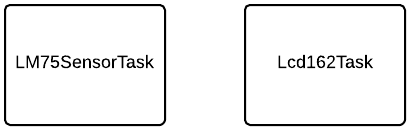
\includegraphics[scale=1]{Two_tasks}
\caption{Systemets tasks}
\label{fig:two-tasks}
\end{figure}



\end{document} 